%!TEX root=ricardo_draft.tex
We begin by describing the problem of fair prediction and introduce three of the most popular definitions developed for this task.  We then give background on causal modeling which will act as our `tool-kit' for modeling and defining fairness.

\subsection{Fairness}
Let's imagine a scenario in which predictions must be fair. For instance, imagine a university in the United States (US) would like to know how successful an applicant is going to be after graduation, call this $Y$, given their current incoming features $X$ such as test scores, grade-point average (GPA). To predict success a modeler is given a dataset of $n$ applications with features $\{X^{(1)}, \ldots, X^{(n)} \}$ and measures of graduation success $\{Y^{(1)}, \ldots, Y^{(n)}\}$. However, universities in the US have historically had racial and gender biases in student admission \cite{kane1998racial,kidder2000portia}. Thus, in addition we are given demographic and gender information for each individual $\{A^{(1)}, \ldots, A^{(n)}\}$ that we would like to use to ensure our model is fair.

What does it mean for a model to be fair? To answer this there has been a wealth of recent work aimed at defining fairness (CITE PAPERS). A few popular definitions are (a) Fairness Through Unawareness (FTU), (b) Demographic Parity (DP), (c) Equal Opportunity (EO), and (d) Individial Fairness (IF). These are defined as follows:

\begin{define}[Fairness Through Unawareness (FTU)]
An algorithm is fair so long as the sensitive attribute $A$ is not explitictly used in the decision-making process. Formally, any mapping $\hat{Y}: X \rightarrow Y$ satisfies this definition.
\end{define}

\begin{define}[Demographic Parity (DP)]
An algorithm is fair if its predictions are independent of the sensitive attributes $A$ across the population. Formally, a prediction $\hat{Y}$ satisfies this definition if, 
\begin{align}
P(\hat{Y} | A = 0) = P(\hat{Y} | A = 1). \nonumber
\end{align}
\end{define}

\begin{define}[Equal Opportunity (EO)]
An algorithm is fair if it is equally accurate for every value of the sensitive attribute $A$. Formally, a prediction $\hat{Y}$ satisfies this if,
\begin{align}
P(\hat{Y}=1 | A=0,Y=1) = P(\hat{Y}=1 | A=1,Y=1). \nonumber
\end{align}
\end{define}

\begin{define}[Individual Fairness (IF)]
An algorithm is fair if it give similar predictions to similar individuals. Formally, if individuals $i$ and $j$ are similar then $\hat{Y}(X^{(i)}, A^{(i)}) \approx \hat{Y}(X^{(j)}, A^{(j)})$.
\end{define}


\subsection{Causal Models and Counterfactuals}
\label{subsec:cmc}
We will follow the framework of \cite{pearl:00}, where a causal
model is a triple $(U, V, F)$ of sets such that
\begin{itemize}
\item $U$ is a set of {\bf background} variables\footnote{These are
  sometimes called {\bf exogeneous variables}, but the fact that members of $U$
  might depend on each other is not relevant to what follows.}, which are generated by factors
outside of our potential control;
\item $V$ is a set of {\bf endogenous} variables, where each member is determined by
  other variables in $U \cup V$;
\item $F$ is a set of functions $\{f_1, \dots, f_n\}$, one for each $V_i \in V$, such
that $V_i = f_i(pa_i, U_{pa_i})$, $pa_i \subseteq V \backslash
\{V_i\}$ and $U_{pa_i} \subseteq U$. Such equations are also known as
{\bf structural equations} \citep{bol:89}.
\end{itemize}

The notation ``$pa_i$'' is motivated by the extra assumption that the
model factorizes according to a directed acyclic graph (DAG). That is,
define a directed graph $\mathcal G$ where each node corresponds to an
element of $U \cup V$, and each edge $V_i \leftarrow X$ is added if
and only if $X \in pa_i \cup U_{pa_i}$. We assume $\mathcal G$ is
acyclic.

The model is causal in the sense that, for a given probability model
$p(U)$ for the background variables, it entails the distribution of a
subset of $V$ given an {\bf intervention} in another subset of $V$.
The operational meaning of an intervention on $V_i$ at value $v$ is
the substitution of the equation $V_i = f_i(pa_i, U_{pa_i})$ with the
equation $V_i = v$. This captures the idea of an agent modifying a
system while being external to it. For instance, this can happen as a
randomized controlled trial that overrides the value of $V_i$ with a
treatment that sets it at $v$, a value chosen at random independently
of any other causes of the system. Pearl's do-calculus
\citep{pearl:00} provides a way of identifying features of 
interventional distributions, when possible, using only (estimates of) the joint
distribution of $V$ and the causal DAG.

Compared to independence constraints given by a DAG, the full
specification of $F$ requires much stronger assumptions but also leads
to much more specific claims. In particular, it allows for the
calculation of {\bf counterfactual} quantities. Without going into a
detailed coverage of the topic, consider the following counterfactual
statement, ``the value of $Y$ had $X$ been $x$'', for two endogenous
variables $X$ and $Y$ in a causal model. By assumption, the state of
any endogenous variable is fully determined by
the background variables and structural equations. The counterfactual is
modeled as the solution for $Y$ for a given $U = u$ where the equation(s)
for $X$ is (are) replaced with $X = x$.  We denote it by $Y_{X \leftarrow x}(u)$
\cite{pearl:00}.

Counterfactual inference, as specified by a causal model $(U, V, F)$,
is the computation of probabilities $P(Y_{X \leftarrow x}(U)\ |\ W =
w)$, where $W$, $X$ and $Y$ are subsets of $V$. Inference proceeds in
three steps, as explained in more detail in Chapter 4 of
\cite{pearl:16}:
\begin{enumerate}
\item For a given prior on $U$, compute the posterior distribution of $U$ given the evidence $W = w$;
\item Substitute the equations for $X$ with the interventional values $x$, resulting
     in the modified set of equations $F_x$;
\item Compute the implied distribution on the remaining elements of $V$
     using $F_x$ and the posterior $P(U\ | W = w)$.
\end{enumerate}


\begin{figure*}[th!]
\begin{center}
\vspace{-2ex}
\centerline{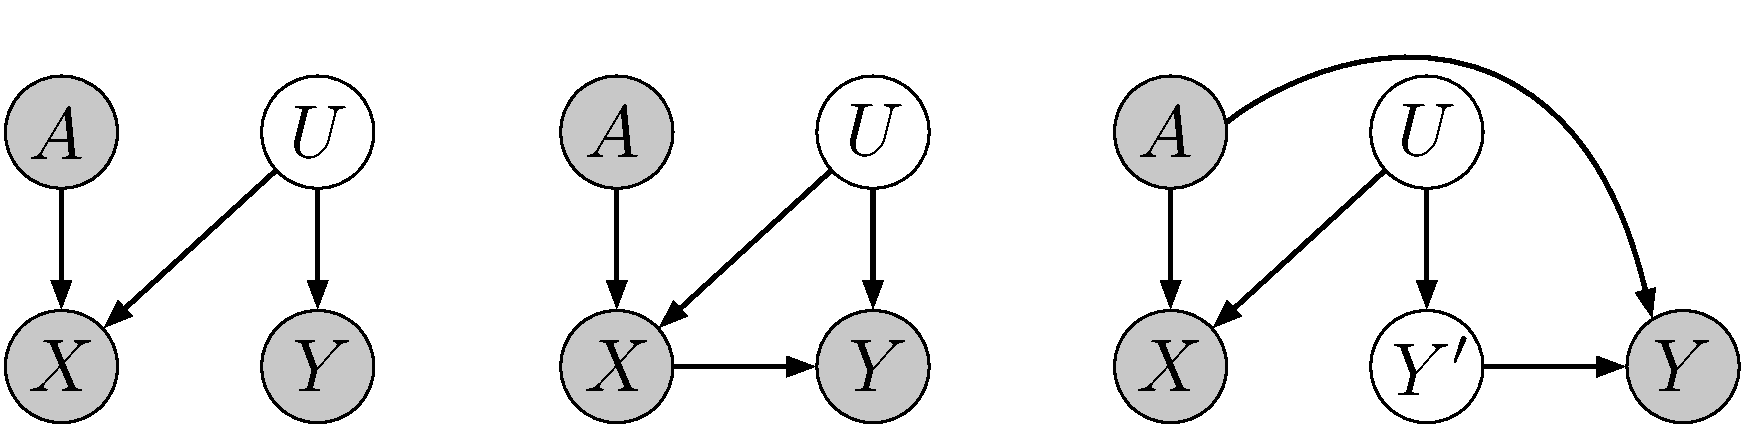
\includegraphics[width=\textwidth]{simple_models_no_q}}
\vspace{-2ex}
\caption{Three possible states of the world.\label{figure.simple_models}}
\vspace{-2ex}
\end{center}
\end{figure*}